% TODO: explain contraction, revision, expansion
% ANSWER: Ich würdes es ganz kurz erläutern im Text. Im Vortrag vielleicht nicht umbedingt.

% TODO QUESTION: do we need to discuss this in ore detail? faithful assignment here:

% ANSWER: Das ist eine gute Frage. So wie ich das Paper von Booth und Meyer im
% Kopf habe werden dort die Ordnung mit epistemischen Zuständen
% gleichgesetzt (was Darwiche und Pearl ja nicht machen). Von daher halte
% ich das für ok es nicht im aller formalen Ausführlichkeit zu machen.
% Aber man könnte es im einen Satz erwähnen.

\documentclass[11pt]{beamer}
\usepackage[utf8]{inputenc}
\usepackage{pgfpages}
\usepackage{amsmath}
\usepackage{amsthm}
\usepackage{amssymb}
\usepackage{dsfont}
\usepackage{tikz}
\usepackage{pgfplots}
\usepackage{float}
\usepackage{stmaryrd}

\usepackage{enumitem}
\setitemize{label=\usebeamerfont*{itemize item}
  \usebeamercolor[fg]{itemize item}
  \usebeamertemplate{itemize item}}

\newcommand{\modelsOf}[1]{\llbracket #1 \rrbracket}

\usefonttheme{professionalfonts}
\usetheme{Madrid}
\usecolortheme{orchid}

\setbeamertemplate{caption}[numbered]
\setbeamertemplate{theorems}[numbered]

% Notes
% Talk using pympress: brew install pympress
% Talk command: pympress -t 40 -n right ~/Documents/master/1901/presentation/1901_3230880_philip_heltweg_presentation.pdf
\setbeameroption{show notes on second screen=right} % Both
% Coloring note-pages
\setbeamertemplate{note page}{\pagecolor{yellow!15}\insertnote\vfill\insertframenumber}
\setbeamertemplate{note page}{
	\pagecolor{yellow!15}
	\medskip
	SLIDE: \insertframenumber\\
	TITLE: \insertframetitle,

	\insertnote
	
}

\AtBeginSection[]
{
  \begin{frame}
    \frametitle{Table of Contents}
    \tableofcontents[currentsection]
  \end{frame}
}

\begin{document}
\title{Of judges, aliens and total preorders}
\author[Heltweg, Philip]{Heltweg, Philip\\pheltweg@gmail.com}
\institute{University of Hagen}
\date{\today}

\frame{\titlepage}

\begin{frame}{Table of Contents}
    \tableofcontents
    
    \note{
        \begin{itemize}
            \item Foo
            \item Bar
        \end{itemize}
    }
\end{frame}

\section{Introduction}

\begin{frame}{Motivation}
    How should a judge change their worldview when presented with new information?  
    \note{
        \begin{itemize}
            \item Example question to motivate
        \end{itemize}
    }
\end{frame}

\begin{frame}{Courtroom example \footnote{inspired by \cite{Booth2011}, \cite{Darwiche1997}}}
    \begin{itemize}
        \item The agent is a judge in a murder trial, "John" and "Mary" are suspects
        \item $\Sigma = \{ p, q, r\}$
        \begin{itemize}
            \item p = "John is the murderer"
            \item q = "Mary is the murderer"
            \item r = "The victim is an alien"
        \end{itemize}
        \item  $I_{\Sigma} = W = \{ 000, 001, 010, 011, 100, 101, 110, 111\}$ 
    \end{itemize} 
    \note{
        \begin{itemize}
            \item NOTE
        \end{itemize}
    }
\end{frame}

\begin{frame}{Research Context}
    \note{
        \begin{itemize}
            \item Research context with areas according to darwiche
        \end{itemize}
    }
\end{frame}

\begin{frame}{Different types of belief}
    \note{
        \begin{itemize}
            \item belief sets (AGM) vs conditional beliefs (Darwiche and Pearl) vs iterating on conditional beliefs (Booth and Meyer)
        \end{itemize}
    }
\end{frame}

\begin{frame}{Paper goal}
    \note{
        \begin{itemize}
            \item present paper goal as defining postulates for a family of operators, functions $\ast$ for iterating on belief change revision operators
            \item explain the concept of defining postulates for a family of operators and research in these postulates to have something to talk about, explain there are different operators and different postulates. this is not finding "the true one" but defining families and discussing pro/contra
        \end{itemize}
    }
\end{frame}

\section{Formal Background}

\begin{frame}{Total preorders}
    \begin{itemize}
        \item Common tool to handle preference orderings over propositional worlds \cite{Booth2011}
        \item binary relation $\leq$, total, reflexive, transitive
        \item  $<$ strict, $\sim$ symmetric closure
    \end{itemize}
    \note{
        \begin{itemize}
            \item total (for all $x, y \in W$ either $x \leq y$ or $y \leq x$)
            \item reflexive ($x \leq x$ for all $x \in W$)
            \item transitive (if $x \leq y$ and $y \leq z$ then $x \leq z$)
            \item  $<$ strict part of $\leq$
            \item $\sim$ symmetric closure of $\leq$ (i.e. $x \sim y$ iff $x \leq y$ and $y \leq x$)
        \end{itemize}
    }
\end{frame}

\begin{frame}{Preorder example}
    \begin{itemize}
        \item Judge beliefs
        \begin{itemize}
            \item Murderer probably acted alone but possible that they conspired
            \item Unlikely, but not impossible, for the victim to be an alien
        \end{itemize} 
        \item $\leq$ over $W$: $010 \sim 100 < 000 \sim 110 < 011 \sim 101 < 001 \sim 111$
    \end{itemize}
    \note{
        \begin{itemize}
            \item NOTE
        \end{itemize}
    }
\end{frame}

\begin{frame}{Preorder visualisation}
    \begin{table}[H]
         \centering
        \begin{tabular}{llll}
        $R_{1}$                      & $R_{2}$                                                                   & $R_{3}$ & $R_{4}$                      \\ \hline
        \multicolumn{1}{|l|}{\begin{tabular}[c]{@{}l@{}}$010$\\ $100$\end{tabular}} & \multicolumn{1}{l|}{\begin{tabular}[c]{@{}l@{}}$000$\\ $110$\end{tabular}} & \multicolumn{1}{l|}{\begin{tabular}[c]{@{}l@{}}$011$\\ $101$\end{tabular}} &
            \multicolumn{1}{l|}{\begin{tabular}[c]{@{}l@{}}$001$\\ $111$\end{tabular}} \\ \hline
        \end{tabular}
        \caption{Visualising a tpo as a linearly ordered set of ranks, as done in \cite{Booth2006}}.
        \label{tab:visualising-a-tpo-example}
    \end{table}
    \note{
        \begin{itemize}
            \item It uses the fact that tpos can be represented as a linearly ordered set of ranks. Each rank of a tpo $\leq$ is defined as the equivalence classes modulo the symmetric closure of $\leq$: $[[x]]_{\sim} = \{y \mid y \sim x\}$. These equivalence classes are then ordered by the relation $[[x]] \leq [[y]]$ iff $x \leq y$.
        \end{itemize}
    }
\end{frame}

\begin{frame}{Belief Sets}
    \note{
        \begin{itemize}
            \item 
        \end{itemize}
    }
\end{frame}

\begin{frame}{Epistemic States}
    \note{
        \begin{itemize}
            \item how to extract belief sets from epistemic states
        \end{itemize}
    }
\end{frame}

\begin{frame}{Belief Set Revision Postulates\footnote{AGM postulates \cite{Alchourron1985}, reformulated for epistemic states by Darwiche and Pearl \cite{Darwiche1997}}}
    \begin{enumerate}[wide=0pt, widest=99,leftmargin=\parindent,label = ($\mathbb{E}\!*\!\arabic*$)]
        \item\label{E1} $\qquad B(\mathbb{E}\ast\alpha) = Cn(B(\mathbb{E}\ast\alpha))$
        \item\label{E2} $\qquad \alpha \in B(\mathbb{E}\ast\alpha)$
        \item\label{E3} $\qquad B(\mathbb{E}\ast\alpha)  \subseteq B(\mathbb{E})+\alpha$
        \item\label{E4} $\qquad \textrm{If } \alpha \notin B(\mathbb{E}) \textrm{ then } B(\mathbb{E}) + \alpha \subseteq B(\mathbb{E} \ast \alpha)$
        \item\label{E5} $\qquad \textrm{If } \mathbb{E} = \mathbb{F} \textrm{ and } \alpha \equiv \beta \textrm{ then } B(\mathbb{E} \ast \alpha) = B(\mathbb{F} \ast \beta)$
        \item\label{E6} $\qquad \bot \in B(\mathbb{E} \ast \alpha) \textrm{ iff } \models \neg \alpha$
        \item\label{E7} $\qquad B(\mathbb{E} \ast (\alpha \wedge \beta)) \subseteq B(\mathbb{E} \ast \alpha) + \beta$
        \item\label{E8} $\qquad \textrm{If } \neg \beta \notin B(\mathbb{E} \ast \alpha) \textrm{ then } B(\mathbb{E} \ast \alpha) + \beta \subseteq B(\mathbb{E} \ast (\alpha \wedge \beta))$
    \end{enumerate}
    
    \note{
        \begin{itemize}
            \item 
        \end{itemize}
    }
\end{frame}

\begin{frame}{Conditional Belief Revision Postulates\footnote{by Darwiche and Pearl \cite{Darwiche1997}}}
    \begin{enumerate}[wide=0pt, widest=99,leftmargin=\parindent,label = (CR$\arabic*$)]
        \item\label{CR1} $\qquad \textrm{If } v\in \modelsOf{\alpha}, w \in \modelsOf{\alpha} \textrm{ then } v \leq_{\mathbb{E}} w \textrm{ iff } v \leq_{\mathbb{E\ast\alpha}} w$
        \item\label{CR2} $\qquad \textrm{If } v\in \modelsOf{\neg\alpha}, w \in \modelsOf{\neg\alpha} \textrm{ then } v \leq_{\mathbb{E}} w \textrm{ iff } v \leq_{\mathbb{E\ast\alpha}} w$
        \item\label{CR3} $\qquad \textrm{If } v\in \modelsOf{\alpha}, w \in \modelsOf{\neg\alpha} \textrm{ then } v <_{\mathbb{E}} w \textrm{ only if } v <_{\mathbb{E\ast\alpha}} w$
        \item\label{CR4} $\qquad \textrm{If } v\in \modelsOf{\alpha}, w \in \modelsOf{\neg\alpha} \textrm{ then } v \leq_{\mathbb{E}} w \textrm{ only if } v \leq_{\mathbb{E\ast\alpha}} w$
    \end{enumerate}
    \note{
        \begin{itemize}
            \item 
        \end{itemize}
    }
\end{frame}

\section{Additional metadata for tpo revision}

\begin{frame}{Enriching Epistemic States}
    \begin{itemize}
        \item $W^{\pm} = \{x^{\epsilon} \mid x \in W \textrm{ and } \epsilon \in \{+, -\}\}$
        \item $w \in \modelsOf{\alpha}$ / $w \in \modelsOf{\neg\alpha}$
        \item $(w^{+}, w^{-})$
    \end{itemize}
    \note{
        \begin{itemize}
            \item W+-
        \end{itemize}
    }
\end{frame}

\begin{frame}{$\leq$-faithful tpo}
    \begin{definition}[$\leq$-faithful tpo over $W^{\pm}$ \cite{Booth2011}]
        \label{definition:faithful-tpo}Let $\preceq \subseteq W^{\pm} \times W^{\pm}$. If $\preceq$ satisfies \ref{PREQ1}-\ref{PREQ4}, we say $\preceq$ is a $\leq$-faithful tpo (over $W^{\pm}$).
    \end{definition}
    \note{
        \begin{itemize}
            \item characteristics + definition
        \end{itemize}
    }
\end{frame}

\begin{frame}[fragile]{$\leq$-faithful tpo visualisation}
    \begin{figure}[H]
        \centering
        \begin{tikzpicture}[scale=1]
            \begin{axis}[
                  yticklabels={,,$x_{4}$,$x_{3}$,$x_{2}$,$x_{1}$},
                  xticklabels={,,},
                  ytick style={draw=none},
                  xtick style={draw=none},
                  axis line style={draw=none}
            ]
            \addplot[
                scatter,
                scatter src=explicit symbolic,
                mark size=3,
                scatter/classes={
                    empty={mark=*, fill=white},
                    filled={mark=*, fill=black}
                },
                nodes near coords*={\Label},
                visualization depends on={value \thisrow{label} \as \Label}
            ]
            table [meta=class] {
                    x y class label
                    
                    3 1 empty $x_{4}^{+}$
                    6 1 empty $x_{4}^{-}$
                                        
                    2 2 empty $x_{3}^{+}$
                    5 2 empty $x_{3}^{-}$
                    
                    1 3 empty $x_{2}^{+}$
                    3 3 empty $x_{2}^{-}$
                    
                    1 4 empty $x_{1}^{+}$
                    3 4 empty $x_{1}^{-}$
            };
            \end{axis}
        \end{tikzpicture}
        \caption{Representation of $\preceq$ over $W^{\pm}$ using intervals}
        \label{fig:example-visualisation-scatterplot}
    \end{figure}
    
    \note{
        \begin{itemize}
            \item example with sticks
        \end{itemize}
    }
\end{frame}

\begin{frame}[fragile]{Courtroom example: $\leq$-faithful tpo}
   \begin{figure}[H]
            \centering
            \begin{tikzpicture}[scale=1]
                \begin{axis}[
                        xticklabels={},
                        yticklabels={},
                        extra y ticks={1, 2, 3, 4, 5, 6, 7, 8},
                        extra y tick labels={$111$, $001$, $101$, $011$, $110$, $000$, $100$, $010$},
                        ytick style={draw=none},
                        xtick style={draw=none},
                        axis line style={draw=none}
                ]
                \addplot[
                    scatter,
                    scatter src=explicit symbolic,
                    mark size=3,
                    scatter/classes={
                        empty={mark=*, fill=white},
                        filled={mark=*, fill=black}
                    },
                    nodes near coords*={\Label},
                    visualization depends on={value \thisrow{label} \as \Label}
                ]
                table [meta=class] {
                        x y class label
                        
                        1 8 empty \empty
                        3 8 empty
                        
                        1 7 empty 
                        3 7 empty
                        
                        2 6 empty 
                        4 6 empty
                        
                        2 5 empty 
                        4 5 empty
                        
                        5 4 empty 
                        7 4 empty
                        
                        5 3 empty 
                        7 3 empty
                        
                        6 2 empty 
                        8 2 empty
                        
                        6 1 empty 
                        8 1 empty
                        };
                \end{axis}
            \end{tikzpicture}
            \caption{Representation of $\preceq$ over $W^{\pm}$ for the courtroom example \ref{example:example-introduction}}
            \label{fig:example-tpo-initial}
    \end{figure}
    
    \note{
        \begin{itemize}
            \item example for courtroom
        \end{itemize}
    }
\end{frame}

\section{Booth and Meyer tpo-revision operators}

\begin{frame}{BM tpo-revision operator}
    \begin{definition}[Revision operator $\ast_{\preceq}$ for $\leq$ generated by $\preceq$ \cite{Booth2011}]
        \label{definition:revision-operator}
        For each $\leq$-faithful tpo $\preceq$ over $W^{\pm}$, refer to $\ast_{\preceq}$ as the revision operator for $\leq$ generated by $\preceq$ defined by:
        
        Set for any $\alpha \in L$ and $x \in W$:
        \begin{equation*}
            r_{\alpha}(x) = \left\{
                        \begin{array}{ll}
                          x^{+} \textrm{ if } x \in \modelsOf{\alpha}\\
                          x^{-} \textrm{ if } x \in \modelsOf{\neg\alpha}
                        \end{array}
                      \right.
        \end{equation*}
        
        The revised tpo $\leq_{\alpha}^{\ast}$ is defined by setting, for each $x, y \in W$,
    
        \begin{equation*}
            x \leq_{\alpha}^{\ast} y \textrm{ iff } r_{\alpha}(x) \preceq r_{\alpha}(y)
        \end{equation*}
    \end{definition}

    \note{
        \begin{itemize}
            \item definition
        \end{itemize}
    }\include{figures/example-visualisation-scatterplot}
\end{frame}

\begin{frame}[fragile]{Courtroom example: Revision Visualised}
    
    \begin{figure}[H]
            \centering
            \begin{tikzpicture}[scale=1]
                \begin{axis}[
                        xticklabels={},
                        yticklabels={},
                        extra y ticks={1, 2, 3, 4, 5, 6, 7, 8},
                        extra y tick labels={$111$, $001$, $101$, $011$, $110$, $000$, $100$, $010$},
                        ytick style={draw=none},
                        xtick style={draw=none},
                        axis line style={draw=none}
                ]
                \addplot[
                    scatter,
                    scatter src=explicit symbolic,
                    mark size=3,
                    scatter/classes={
                        empty={mark=*, fill=white},
                        filled={mark=*, fill=black}
                    },
                    nodes near coords*={\Label},
                    visualization depends on={value \thisrow{label} \as \Label}
                ]
                table [meta=class] {
                        x y class label
                        
                        1 8 empty \empty
                        3 8 filled
                        
                        1 7 filled 
                        3 7 empty
                        
                        2 6 empty 
                        4 6 filled
                        
                        2 5 filled 
                        4 5 empty
                        
                        5 4 empty 
                        7 4 filled
                        
                        5 3 filled 
                        7 3 empty
                        
                        6 2 empty 
                        8 2 filled
                        
                        6 1 filled 
                        8 1 empty
                        };
                \end{axis}
            \end{tikzpicture}
            \caption{Associating positive and negative representations of worlds after receiving evidence $\alpha=p$}
            \label{fig:example-tpo-revised}
    \end{figure}
    
    \note{
        \begin{itemize}
            \item example 7, figure 4
        \end{itemize}
    }
\end{frame}

\begin{frame}{Courtroom example: Revision}

    \begin{itemize}
        \item for $010, 110 \in W$, $010 \leq 110$ before, revise by $\alpha = p$
    \end{itemize}

    \begin{equation*}
        010 \in \modelsOf{\neg\alpha} \textrm{ : } r_{\alpha}(010) = 010^{-}
    \end{equation*}
    \begin{equation*}
        110 \in \modelsOf{\alpha} \textrm{ : } r_{\alpha}(110) = 110^{+}
    \end{equation*}
    
    \begin{itemize}
        \item $110^{+} \prec 010^{-}$ is true, set $110 <_{\alpha}^{\ast} 010$
        \item new tpo $\leq_{\alpha}^{\ast}$ is: $100 <_{\alpha}^{\ast} 110 <_{\alpha}^{\ast} 010 <_{\alpha}^{\ast} 000 <_{\alpha}^{\ast} 101 <_{\alpha}^{\ast} 111 <_{\alpha}^{\ast} 011 <_{\alpha}^{\ast} 001$
        \item $\modelsOf{B(\mathbb{E})} = min(\top, \leq_{\mathbb{E}}) = \{100\}$: "John is the murderer and the victim is not an alien".
        \item $\leq_{\alpha}^{\ast}$ as representation of the conditional beliefs
        \begin{itemize}
            \item before $010 \leq 110$: "Both suspects being the murderer is less plausible than Mary being the murderer"
            \item now $110 <_{\alpha}^{\ast} 010$: "Only Mary being the murderer less plausible than both conspiring".
        \end{itemize}
    \end{itemize}
    
    \note{
        \begin{itemize}
            \item example 7, math
        \end{itemize}
    }
\end{frame}


\begin{frame}{BACKUP: non-prioritised revision}
    \note{
        \begin{itemize}
            \item example 7, figure 4
        \end{itemize}
    }
\end{frame}

\begin{frame}{Properties of BM Revision Operators}
    \begin{enumerate}[wide=0pt, widest=99,leftmargin=\parindent,label = ($\ast\arabic*$)]
        \item\label{AST1} $\qquad \leq_{\alpha}^{\ast} \textrm{ is a tpo over } W$
        \item\label{AST2} $\qquad\alpha \equiv \gamma \textrm{ implies } \leq_{\alpha}^{\ast}=\leq_{\gamma}^{\ast}$
        \item\label{AST3} $\qquad \textrm{If } x, y \in \modelsOf{\alpha} \textrm{ then } x \leq_{\alpha}^{\ast} y \textrm{ iff } x \leq y$
        \item\label{AST4} $\qquad \textrm{If } x, y \in \modelsOf{\neg\alpha} \textrm{ then } x \leq_{\alpha}^{\ast} y \textrm{ iff } x \leq y$
        \item\label{AST5} $\qquad \textrm{If } x \in \modelsOf{\alpha}, y \in \modelsOf{\neg\alpha} \textrm{ and } x \leq y \textrm{ then } x <_{\alpha}^{\ast} y$
        \item\label{AST6} $\qquad \textrm{If } x \in \modelsOf{\alpha}, y \in \modelsOf{\neg\alpha} \textrm{ and } y \leq_{\alpha}^{\ast} x \textrm{ then } y \leq_{\gamma}^{\ast} x$
        \item\label{AST7} $\qquad \textrm{If } x \in \modelsOf{\alpha}, y \in \modelsOf{\neg\alpha} \textrm{ and } y <_{\alpha}^{\ast} x \textrm{ then } y <_{\gamma}^{\ast} x$
    \end{enumerate}

    \note{
        \begin{itemize}
            \item properties
        \end{itemize}
    }
\end{frame}

\begin{frame}{Family of BM Revision Operators}
    \begin{theorem}
        \label{theorem:revision-operator}Let $\ast$ be any revision operator for $\leq$. Then $\ast$ is generated from some $\leq$-faithful tpo $\preceq$ over $W^{\pm}$ iff $\ast$ satisfies \ref{AST1}-\ref{AST7}. \cite{Booth2011}
    \end{theorem}

    \note{
        \begin{itemize}
            \item theorem 1
        \end{itemize}
    }
\end{frame}

\section{Iterating: $\preceq$-revision}

\begin{frame}{A concrete operator}
    \begin{itemize}
        \item $p: W^{\pm} \mapsto \mathds{R}$
        \item $p(x^{-}) - p(x^{+}) = a > 0$
        \item $x^{\epsilon} \preceq_{p} y^{\delta} \textrm{ iff } p(x^{\epsilon}) \leq p(y^{\delta})$
        \item Set $p$, for every $x^{\epsilon} \in W^{\pm}$, to:
    \end{itemize}
    
    \begin{equation*}
        (p \ast \alpha)(x^{\epsilon}) = \left\{
                        \begin{array}{ll}
                          p(x^{\epsilon}) \textrm{ if } x \in \modelsOf{\alpha}\\
                          p(x^{\epsilon}) + a \textrm{ if } x \in \modelsOf{\neg\alpha}
                        \end{array}
                      \right.
    \end{equation*}
    
    \note{
        \begin{itemize}
            \item math for operator
        \end{itemize}
    }
\end{frame}

\begin{frame}{Courtroom Example: A concrete operator}
    \begin{itemize}
        \item Choose initial $p$ so that $\preceq_{p} = \preceq$
        \begin{itemize}
            \item $010 \textrm{ : } (p(010^{+}), p(010^{-})) = (0, a)$.
            \item $100 \textrm{ : } (p(100^{+}), p(100^{-})) = (0, a)$.
        \end{itemize}
        \item Revise $p$ by $\alpha$ to $p \ast \alpha$
        \begin{itemize}
            \item $010 \in \modelsOf{\neg\alpha} \textrm{ : } (p(010^{-}), p(010^{-}) + a) = (a, 2a)$
            \item $100 \in \modelsOf{\alpha} \textrm{ : } (p(100^{+}), p(100^{-})) = (0, a)$
        \end{itemize}
            \end{itemize}

    \note{
        \begin{itemize}
            \item math for example with operator
        \end{itemize}
    }
\end{frame}

\begin{frame}[fragile]{Courtroom Example: Visualised}
    \begin{figure}[H]
            \centering
            \begin{tikzpicture}[scale=1]
                \begin{axis}[
                        xticklabels={},
                        yticklabels={},
                        extra y ticks={1, 2, 3, 4, 5, 6, 7, 8},
                        extra y tick labels={$111$, $001$, $101$, $011$, $110$, $000$, $100$, $010$},
                        ytick style={draw=none},
                        xtick style={draw=none},
                        axis line style={draw=none}
                ]
                \addplot[
                    scatter,
                    scatter src=explicit symbolic,
                    mark size=3,
                    scatter/classes={
                        empty={mark=*, fill=white},
                        old={mark=x, fill=white}
                    },
                    nodes near coords*={\Label},
                    visualization depends on={value \thisrow{label} \as \Label}
                ]
                table [meta=class] {
                        x y class label
                        
                        1 8 old \empty
                        
                        3 8 empty
                        5 8 empty 
                        
                        1 7 empty 
                        3 7 empty
                        
                        2 6 old 
                        
                        4 6 empty
                        6 6 empty
                        
                        2 5 empty 
                        4 5 empty
                        
                        5 4 old 
                        
                        7 4 empty
                        9 4 empty
                        
                        5 3 empty 
                        7 3 empty
                        
                        6 2 old 
                        
                        8 2 empty
                        10 2 empty
                        
                        6 1 empty 
                        8 1 empty
                        };
                \end{axis}
            \end{tikzpicture}
            \caption{$\preceq_{p \ast \alpha}$ for $\alpha = p$}
            \label{fig:example-preceq-revised}
    \end{figure}
    
    \note{
        \begin{itemize}
            \item figure 7
        \end{itemize}
    }
\end{frame}

\begin{frame}[fragile]{Courtroom Example: Conditional beliefs 1}
    \begin{figure}[H]
            \centering
            \begin{tikzpicture}[scale=1]
                \begin{axis}[
                        xticklabels={},
                        yticklabels={},
                        extra y ticks={1, 2, 3, 4, 5, 6, 7, 8},
                        extra y tick labels={$111$, $001$, $101$, $011$, $110$, $000$, $100$, $010$},
                        ytick style={draw=none},
                        xtick style={draw=none},
                        axis line style={draw=none}
                ]
                \addplot[
                    scatter,
                    scatter src=explicit symbolic,
                    mark size=3,
                    scatter/classes={
                        empty={mark=*, fill=white},
                        old={mark=x, fill=white}
                    },
                    nodes near coords*={\Label},
                    visualization depends on={value \thisrow{label} \as \Label}
                ]
                table [meta=class] {
                        x y class label
                        
                        1 8 old \empty
                        
                        3 8 empty
                        5 8 empty 
                        
                        1 7 old
                        
                        3 7 empty 
                        5 7 empty
                        
                        2 6 old 
                        
                        4 6 empty
                        6 6 empty
                        
                        2 5 old
                        
                        4 5 empty 
                        6 5 empty
                        
                        5 4 empty
                        7 4 empty
                        
                        5 3 empty 
                        7 3 empty
                        
                        6 2 empty
                        8 2 empty
                        
                        6 1 empty 
                        8 1 empty
                        };
                \end{axis}
            \end{tikzpicture}
            \caption{$\preceq_{p \ast \alpha}$ for $\alpha = r$}
            \label{fig:example-preceq-revised-alien}
    \end{figure}
    
    \note{
        \begin{itemize}
            \item figure 8
        \end{itemize}
    }
\end{frame}

\begin{frame}[fragile]{Courtroom Example: Conditional beliefs 2}
    \begin{figure}[H]
            \centering
            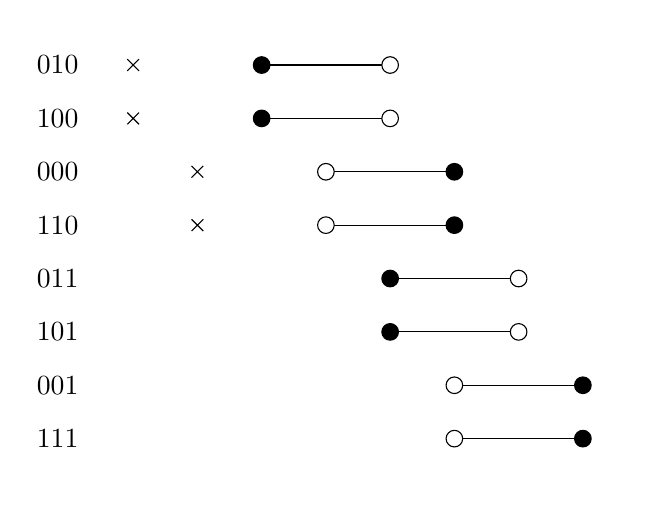
\begin{tikzpicture}[scale=1]
                \begin{axis}[
                        xticklabels={},
                        yticklabels={},
                        extra y ticks={1, 2, 3, 4, 5, 6, 7, 8},
                        extra y tick labels={$111$, $001$, $101$, $011$, $110$, $000$, $100$, $010$},
                        ytick style={draw=none},
                        xtick style={draw=none},
                        axis line style={draw=none}
                ]
                \addplot[
                    scatter,
                    scatter src=explicit symbolic,
                    mark size=3,
                    scatter/classes={
                        empty={mark=*, fill=white},
                        filled={mark=*, fill=black},
                        old={mark=x, fill=white}
                    },
                    nodes near coords*={\Label},
                    visualization depends on={value \thisrow{label} \as \Label}
                ]
                table [meta=class] {
                        x y class label
                        
                        1 8 old \empty
                        
                        3 8 filled
                        5 8 empty 
                        
                        1 7 old
                        
                        3 7 filled 
                        5 7 empty
                        
                        2 6 old 
                        
                        4 6 empty
                        6 6 filled
                        
                        2 5 old
                        
                        4 5 empty 
                        6 5 filled
                        
                        5 4 filled
                        7 4 empty
                        
                        5 3 filled 
                        7 3 empty
                        
                        6 2 empty
                        8 2 filled
                        
                        6 1 empty 
                        8 1 filled
                        };
                \end{axis}
            \end{tikzpicture}
            \caption{$\preceq_{p \ast \alpha \ast \beta}$ for $\beta = (p \vee q) \wedge (\neg p \vee \neg q)$}
            \label{fig:example-preceq-revised-alien2}
    \end{figure}
    
    \note{
        \begin{itemize}
            \item figure 9
        \end{itemize}
    }
\end{frame}

\begin{frame}{}
  \centering \Huge
  Thank You
\end{frame}

\begin{frame}{References}
    \typeout{}
    \bibliographystyle{plain}
    \bibliography{references}
\end{frame}

\end{document}